\section{Theorie}
\label{sec:theorie}

    Im folgenden Abschnitt werden die theoretischen Grundlagen für diesen Versuch erläutert werden.
    Dabei wird zum einen die Wechselwirkung von Gamma-Strahlung mit Materie,
    sowie die Detektion der Strahlung beschrieben.

    Bei dem verwendeten Verfahren der Tomographie wird die zu untersuchende Probe mithilfe von Projektionen schichtweise betrachtet.

\subsection{Wechselwirkung von Gamma-Strahlung mit Materie}

    Gamma-Strahlung besteht aus hochenergetischen Photonen die bei Zerfallsprozessen erzeugt werden.
    In diesem Fall wird der Zerfall des radioaktiven Zerfalls $^{137}\ce{Cs}$ betrachtet,
    welches über einen $\beta$-Zerfall und anschließenden $\gamma$-Zerfall in das stabile $^{137}\ce{Ba}$ zerfällt.
    Dabei wird Strahlung der Energie $E_{\symup{\gamma}} \approx \SI{662}{\kilo\eV}$ \cite{caesium} frei.
    Dieser Prozess ist in \autoref{fig:theorie:zerfallsprozess} dargestellt.

    Wenn die $\gamma$-Strahlung nun auf Materie trifft,
    muss abhängig von der Energie der Strahlung zwischen folgenden Effekten unterschieden werden \cite{radioaktivitaet}.

    \begin{figure}
       \centering
       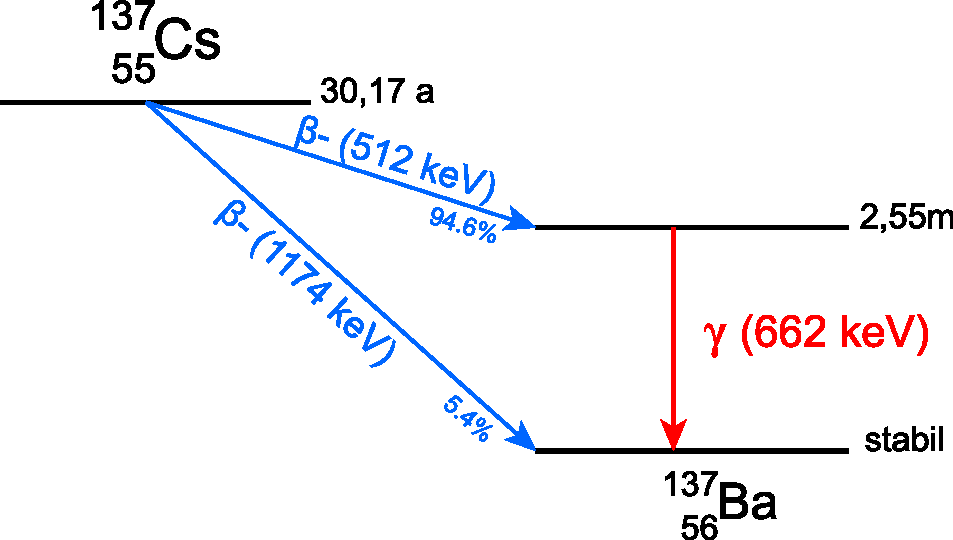
\includegraphics[width=0.5\textwidth]{content/img/zerfallsschema_Leifi.pdf} % TODO: Durch eigene Grafik ersetzen oder Quelle angeben
       \caption{Zerfallsprozess von \ce{^137Cs} in das stabile \ce{^137Ba}. \cite{caesium}}
       \label{fig:theorie:zerfallsprozess}
    \end{figure}

    \label{sec:theorie:photoeffekt}
    Für niedrigere Energien (\%Bereich aus KET) tritt größtenteils der \textbf{Photoeffekt} auf.
    Dabei muss die Energie des Photons $E_{\symup{\gamma}} = hf$ der Bindungsenergie eines der Hüllenelektronen entsprechen.
    Das Photon gibt in diesem Fall seine gesamte Energie an das Elektron ab,
    welches aus dem Atom herausgelöst wird.
    Das Elektron behält dabei eine Energie $E_{e} = hf - E_\text{Bind}$.
    Der Wirkungsquerschnitt unterscheidet sich dabei,
    ob die Energie des Photons kleiner oder größer der relativistischen Ruheenergie des Elektrons ist.
    Es gilt
    \begin{equation*}
        \sigma_\text{Photo} \propto
        \begin{cases}
            \sfrac{Z^5}{E^{\sfrac{7}{2}}_{\symup{\gamma}}} & , E_{\symup{\gamma}} \ll m_{e} c^2 \\
            \sfrac{Z^5}{E_{\symup{\gamma}}} & , E_{\symup{\gamma}} \gg m_{e} c^2 \\
        \end{cases} \ .
    \end{equation*}


    \label{sec:theorie:comptoneffekt}
    Für zunehmende Energien dominiert der \textbf{Compton-Effekt}.
    Das Photon gibt in diesem Fall nicht mehr seine gesamte Energie ab,
    sondern stößt elastisch mit lose gebundenen oder freien Elektronen.
    Dabei gilt Energie- und Impulserhaltung,
    sodass das Photon einen Teil seiner Energie an das Elektron abgibt und beide eine Richtungsänderung erfahren.
    Die Energieabgabe des Photons ist abhängig vom Streuwinkel.
    Das Elektron kann eine maximale Energie erreichen,
    wenn für den Streuwinkel des Photons $\vartheta = \SI{0}{\degree}$ gilt.
    Im Energiespektrum findet sich an diesem Punkt die sogenannte \textit{Compton-Kante}.
    Für den Wirkungsquerschnitt gilt
    \begin{equation*}
        \sigma_\text{Compton} \propto \sfrac{Z}{E_{\symup{\gamma}}} \ .
    \end{equation*}


    \label{sec:theorie:paarerzeugung}
    Für eine Energie $E_{\symup{\gamma}} \geq 2m_{e}c^2 = \SI{1.022}{\mega\eV}$ kann \textbf{Paarerzeugung} stattfinden.
    Dabei wandelt sich das Photon im Coulombfeld des Atoms in ein Elektron-Positron-Paar um.
    Dieser Prozess kann aufgrund der Erhaltungssätze nur mit dem Atomkern als weiteren Stoßpartner stattfinden.
    Die entstehenden Teilchen haben eine Energie von $E_{e^{+}} + E_{e^{-}} = E_{\symup{\gamma}} - 2m_{e}c^2$.
    Weiterhin gilt
    \begin{equation*}
        \sigma_\text{Paar} = Z^2 \ln(E_{\symup{\gamma}}) \ .
    \end{equation*}


    In jedem der Fälle wird die Gamma-Strahlung vom Material absorbiert.
    Dabei ist die Absorption materialabhängig.
    Dies kann über den Absorptionskoeffizienten
    \begin{equation}
        \mu = \sigma \cdot \rho
        \label{eqn:theorie:absorptionskoeffizient}
    \end{equation}
    beschrieben werden,
    wobei $\rho$ die Dichte des Materials und $\sigma = \sigma_\text{Photo} + \sigma_\text{Compton}$ darstellt.
    Die Paarerzeugung kann mit der verwendeten $^{137}\ce{Cs}$-Strahlungsquelle nicht stattfinden,
    da die entsprechende Energie zu gering ist.
    \autoref{tab:theorie:literaturwerte} zeigt die Wirkungsquerschnitte,
    Dichten und Absorptionskoeffizienten von verschiedenen Stoffen.
    \begin{table}[H]
        \centering
        \caption{Absorptionskoeffizient, Dichte und Wirkungsquerschnitte verschiedener Stoffe.
        Der Absorptionskoeffizient wird über \autoref{eqn:theorie:absorptionskoeffizient} berechnet.
        Die Dichten der Stoffe wurden \cite{dichten} und \cite{dichte_delrin} entnommen,
        die Wirkungsquerschnitte aus \cite{crosssections}.}
        \label{tab:theorie:literaturwerte}
        \expandableinput{build/tab/mu.tex}
    \end{table}
    Abhängig vom Material des Stoffes wird die Gammastrahlung bei der Absorption abgeschwächt.
    Dabei fällt die Intensität exponentiell mit der Weglänge ab.
    Für eine Aneinanderreihung von Wegstücken $x_i$
    mit unterschiedlichen Absorptionskoeffizienten $\mu_i$
    ergibt sich für die Intensität
    \begin{align}
        I &= I_0 \exp\Bigl(\sum_{i=1}^N \mu_i x_i \Bigr) \\
        \iff \ln\left(\frac{I}{I_0}\right) &= \sum_{i=1}^N \mu_i x_i \ .
        \label{eqn:theorie:intensitaet2}
    \end{align}
    Mit Bezug auf die Absorptionskoeffizienten kann das lineare Gleichungssystem
    \begin{equation}
        \symbf{A} \cdot \vec{\mu} = \vec{I}
    \end{equation}
    aufgestellt werden,
    wobei $\vec{I}$ die Projektionen durch das Material beschreiben.
    %\begin{figure}
    %    \centering
    %    \includegraphics[witdth=\textwidth]{}
    %    \caption{Projektionen $I$ durch den hier betrachteten 3x3x3 Würfel.}
    %    \label{fig:theorie:projektionen}
    %\end{figure}
    Für die Projektionen,
    die in \autoref{fig:theorie:projektionen} gezeigt sind,
    in diesem Fall durch einen 3x3x3 Würfel,
    ergibt sich mit \autoref{eqn:theorie:intensitaet2} das Gleichungssystem
    \begin{equation}
        \begin{pmatrix}
            I_{147} \\
            I_{258} \\
            I_{369} \\
            I_{789} \\
            I_{456} \\
            I_{123} \\
            I_{24}  \\
            I_{357} \\
            I_{68}  \\
            I_{48}  \\
            I_{159} \\
            I_{26}
        \end{pmatrix}
        = d \cdot
        \begin{pmatrix}
            1        & 0        & 0        & 1        & 0        & 0        & 1        & 0        & 0        \\
            0        & 1        & 0        & 0        & 1        & 0        & 0        & 1        & 0        \\
            0        & 0        & 1        & 0        & 0        & 1        & 0        & 0        & 1        \\
            0        & 0        & 0        & 0        & 0        & 0        & 1        & 1        & 1        \\
            0        & 0        & 0        & 1        & 1        & 1        & 0        & 0        & 0        \\
            1        & 1        & 1        & 0        & 0        & 0        & 0        & 0        & 0        \\
            0        & \sqrt{2} & 0        & \sqrt{2} & 0        & 0        & 0        & 0        & 0        \\
            0        & 0        & \sqrt{2} & 0        & \sqrt{2} & 0        & \sqrt{2} & 0        & 0        \\
            0        & 0        & 0        & 0        & 0        & \sqrt{2} & 0        & \sqrt{2} & 0        \\
            0        & 0        & 0        & \sqrt{2} & 0        & 0        & 0        & \sqrt{2} & 0        \\
            \sqrt{2} & 0        & 0        & 0        & \sqrt{2} & 0        & 0        & 0        & \sqrt{2} \\
            0        & \sqrt{2} & 0        & 0        & 0        & \sqrt{2} & 0        & 0        & 0
        \end{pmatrix}
        \cdot
        \begin{pmatrix}
            \mu_1 \\
            \mu_2 \\
            \mu_3 \\
            \mu_4 \\
            \mu_5 \\
            \mu_6 \\
            \mu_7 \\
            \mu_8 \\
            \mu_9
        \end{pmatrix}
        \ .
    \end{equation}

\subsection{Detektion der Gammastrahlung}

    Zur Detektion der Gamma-Strahlung wird ein \textit{Szintillator} genutzt.
    In diesem werden durch die auftreffende Strahlung Atome angeregt,
    die Licht emittieren.
    Dieses Licht wird mithilfe eines Photomultipliers verstärkt und in Photostrom umgewandelt,
    sodass Lichtimpulse gemessen werden können.
    Da das entstehende Licht proportional zur Energie der einfallenden Strahlung ist,
    kann mithilfe des Szintillators ein Energiespektrum gemessen werden.
    Zudem wird ein \textit{Diskriminator} verwendet.
    Dieser dient dazu,
    Hintergrundsignal auszusortieren,
    welches durch den Photomultiplier oder andere Detektoren entsteht.
    Der Diskriminator legt dazu eine Energieschwelle fest.
    Gemessene Signale,
    deren Energie unter dieser Schwelle liegt,
    werden nicht registriert.
    Mithilfe eines \textit{Multichannel Analysers} werden die gemessenen Impulse ihrer Energie nach geordnet.
